\documentclass{article}
\usepackage{amsmath}
\usepackage[utf8]{inputenc}
\usepackage[margin=2cm]{geometry} 
\usepackage{graphicx}
\usepackage{placeins}
\usepackage[skip=10pt plus1pt, indent=40pt]{parskip}
\usepackage{float}
\usepackage{booktabs}
\usepackage{multicol}
\usepackage{gensymb}
\usepackage{amsmath}
\usepackage{hyperref}
\hypersetup{
    colorlinks=true,
    linkcolor=blue,
    filecolor=blue,
    citecolor=black,
    urlcolor=cyan
    }


\begin{document}
\title{Studio delle oscillazioni accoppiate di due pendoli}
\author{Alessia Di Nino, Alessandra Natì (corso B, gruppo B 1-2)}
\date{30 Marzo 2023}
\maketitle

\section{Introduzione}
\subsection{Cenni Teorici}
L'equazione del moto del pendolo semplice è descritta da:
\begin{equation}
    \Ddot{\theta} = -\frac{mgL}{I} sin \theta
\end{equation}
da cui, a regime di piccole oscillazioni (per cui approssimando $sin \theta \sim \theta$) otteniamo che la pulsazione angolare prevista dalla teoria è:
\begin{equation}
    \omega_0 = \sqrt{\frac{mgl}{I}}
    \label{omega}
\end{equation}
dove I è il momento d'inerzia del pendolo rispetto al punto di sospensione. Considerando l'asta trascurabile rispetto al corpo cilindrico del pendolo, il momento d'inerzia si può misurare tramite il teorema di Huygens Steiner come la somma tra il momento d'inerzia di un cilindro rispetto al proprio centro e la componente che indica la distanza dal punto di sospensione:

\begin{equation}
    I = \frac{1}{2}mR^2 + ml^2
\end{equation}

La legge che governa il moto del pendolo nel caso di aggiunta di uno smorzatore è:

\begin{equation}
    \theta_0(t) = \theta_0(0)e^{\frac{-t}{\tau}}
\end{equation}

con $\tau$ pari al tempo di decadimento dell'ampiezza d'oscillazione (ossia il tempo in cui l'ampiezza dell'oscillazione si riduce di un fattore pari a $\frac{1}{e}$).\\
Nel momento in cui si accoppiano due pendoli (collegandoli con una molla), il moto può risultare in generale molto complicato. Tuttavia esistono due configurazioni iniziali, corrispondenti ai cosiddetti modi normali di oscillazione, per cui il moto di entrambi i pendoli è armonico. Questi corrispondono alle configurazioni in cui i pendoli si muovono in fase ed in controfase.\\
Per far muovere i pendoli in fase, basta spostarli nello stesso verso e di uguali ampiezze, lasciandoli andare nello stesso momento. In queste condizioni la molla non è sollecitata, dunque non influenza il movimento dei due pendoli i quali, infine, oscilleranno con la stessa frequenza che è pari a quella di un pendolo che oscilla da solo. Proprio per questo motivo, infatti, per la teoria $\omega_f \sim \omega_0$, con $\omega_f$ la pulsazione del moto in fase.\\
Per far muovere i pendoli in controfase, invece, bisogna spostarli in versi opposti, ma sempre della stessa ampiezza, sempre a condizione di lasciarli andare contemporaneamente. In questa condizione, differentemente dalla prima, risulta $\omega_c > \omega_f$, anche se, nel caso in cui la costante elastica della molla fosse piccola, la differenza tra le due pulsazioni angolari non sarebbe grande.\\
Tutti i moti possibili dei pendoli accoppiati risultano da una combinazione dei modi normali così isolati. Infatti, un'ulteriore configurazione potrebbe essere quella in cui si lasciano partire i pendoli in modo che uno sia fermo nella sua posizione di equilibrio stabile, mentre l'altro venga spostato di una data ampiezza. Ciò che si ottiene da queste condizioni è il cosiddetto fenomeno dei battimenti, dovuto per l'appunto all'interferenza di oscillazioni di diverso periodo. Il moto risultante è dato dalla somma dei due modi normali ed è così espresso:

\begin{equation}
    x(t) = A_0[cos(\omega_f t + \phi1) + cos(\omega_c t + \phi_2)]
\end{equation}

L'oscillazione risultante viene così caratterizzata da una pulsazione angolare portante pari a:

\begin{equation}
    \omega_p = \frac{\omega_c + \omega_f}{2} \sim \omega_c, \omega_f
\end{equation}

modulata da un'onda sinusoidale di pulsazione angolare modulante molto più piccola (e quindi periodo molto più grande) pari a:

\begin{equation}
    \omega_b = \frac{\omega_c - \omega_f}{2} << \omega_c, \omega_f
\end{equation}

\vspace{1em}

\subsection{Scopo dell'esperienza}
Lo scopo di questa esperienza è lo studio del moto di due pendoli accoppiati quando essi sono in fase ed in controfase, nonchè lo studio del fenomeno dei battimenti; altro scopo dell'esperienza è il confronto del moto di un pendolo che oscilla liberamente con il moto di un pendolo che oscilla con smorzatore.

\vspace{2em}

\section{Metodi}
\subsection{Apparato sperimentale}
Per condurre l'esperimento ci siamo servite di:
\begin{itemize}
    \item due pendoli accoppiati (attraverso una molla);
    \item un galleggiante da pesca (che funge da smorzatore);
    \item un sistema di acquisizione per registrare la posizione di ciascun pendolo in funzione del tempo.
\end{itemize}
In particolare, l'apparato consiste in un supporto su cui sono fissati due pendoli uguali, formati da un cilindro di ottone, un'asta di alluminio e un terminale a forma di ago. Al di sotto dei pendoli è presente una vasca d'acqua in cui sono immersi gli aghi dei pendoli: l'acqua serve ad aumentare l'attrito. Inoltre, tramite un sistema elettrico, è proprio l'ago che trasmette le informazioni al programma di acquisizione da cui abbiamo estratto i dati.

\begin{figure} [H]
    \centering
    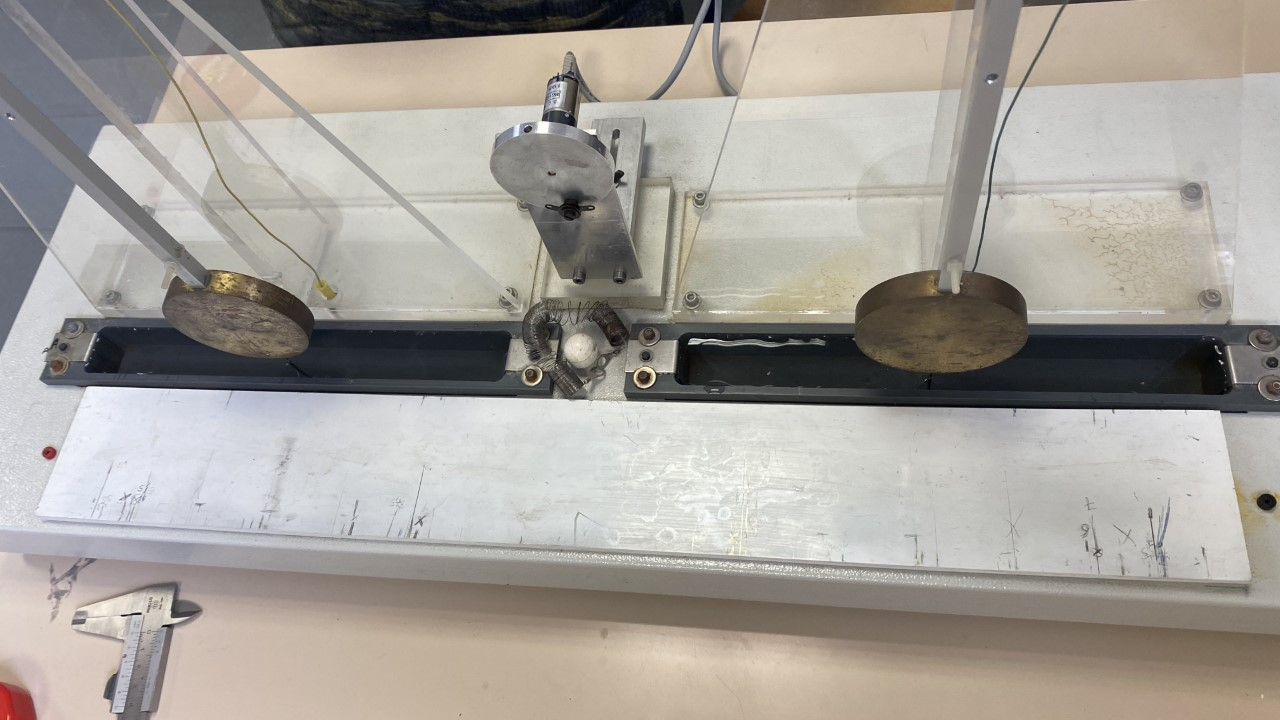
\includegraphics[width=8cm]{pendoli.jpg}
    \caption{Dettaglio dell'apparato sperimentale sulla vasca d'acqua sottostante i due pendoli}
    \label{fig:my_label}
\end{figure}

\begin{figure} [H]
    \centering
    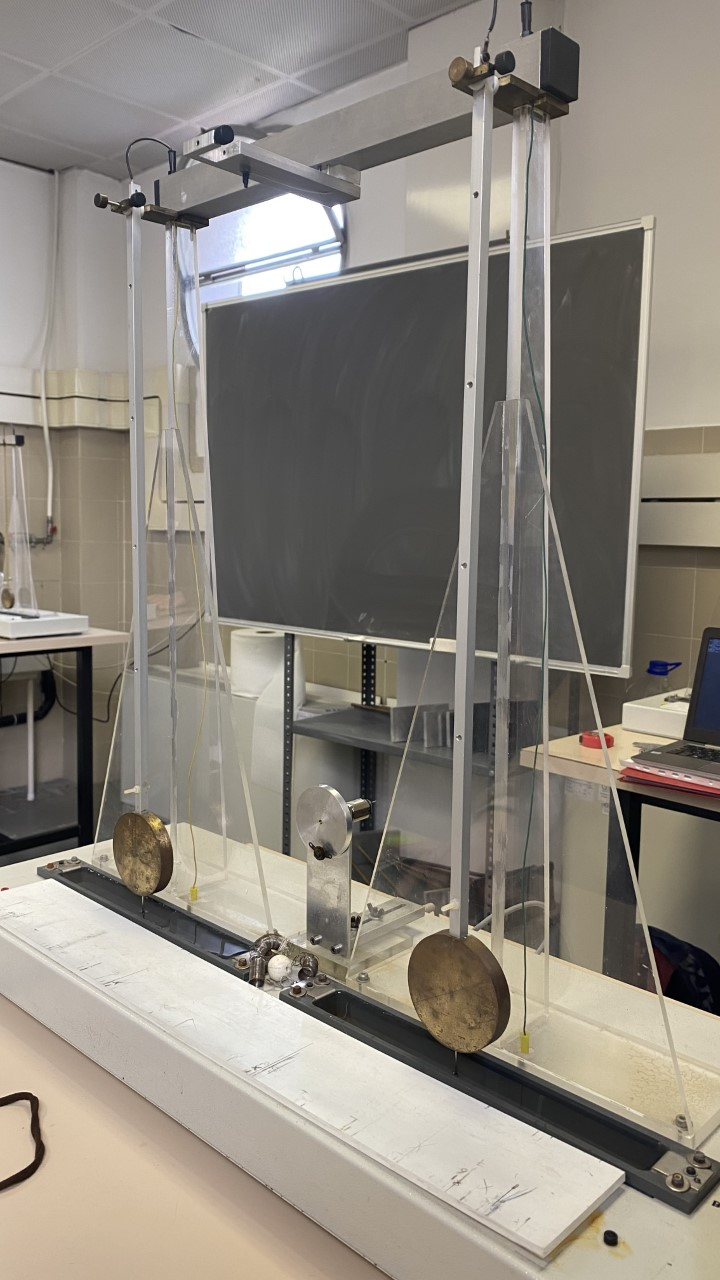
\includegraphics[width=10cm]{coppia.jpg}
    \caption{Apparato sperimentale}
    \label{fig:my_label}
\end{figure}

\FloatBarrier

\vspace{1em}

\subsection{Descrizione delle misure}
Come prima cosa, abbiamo preso le misure delle dimensioni e della massa del pendolo per poter stimare a livello teorico la pulsazione $\omega_0$ tramite la formula \eqref{omega}. Abbiamo dunque misurato il raggio del corpo cilindrico in ottone e la lunghezza tra il punto di sospensione e il centro del cilindro (che corrisponde alla lunghezza di asta + raggio). Considerando la massa dell'asta trascruabile, appunto, rispetto alla massa del corpo cilindrico (in quanto impossibile misurarne la massa separatamente dal resto del corpo del pendolo), si ottiene che il centro di massa del sistema coincide propriamente con il centro del cilindro. Le misure ottenute sono:

\begin{tabular}{ccc}
    \toprule
    R & $(3.5 \pm 0.1) cm$ \\
    l & $(53 \pm 0.1)cm$\\
    m & $(0.465 \pm 0.005)Kg$\\
    \bottomrule
\end{tabular} 

Otteniamo dunque un valore di $\omega_0 = (4.34 \pm 0.01) rad/s$.\\
Di seguito, abbiamo messo in oscillazione uno dei due pendoli, prima semplice e poi smorzata. Lo smorzatore consisteva in un galleggiante da pesca infilato nell'ago che era a contatto con l'acqua. Ovviamente in entrambi i casi l'oscillazione singola risulta smorzata, ma con l'aggiunta del galleggiante è stato aumentato l'attrito per cui lo smorzamento è risultato maggiore.\\
\\
Subito dopo abbiamo accoppiato i due pendoli tramite una molla per isolare i modi normali.

\begin{figure} [H]
    \centering
    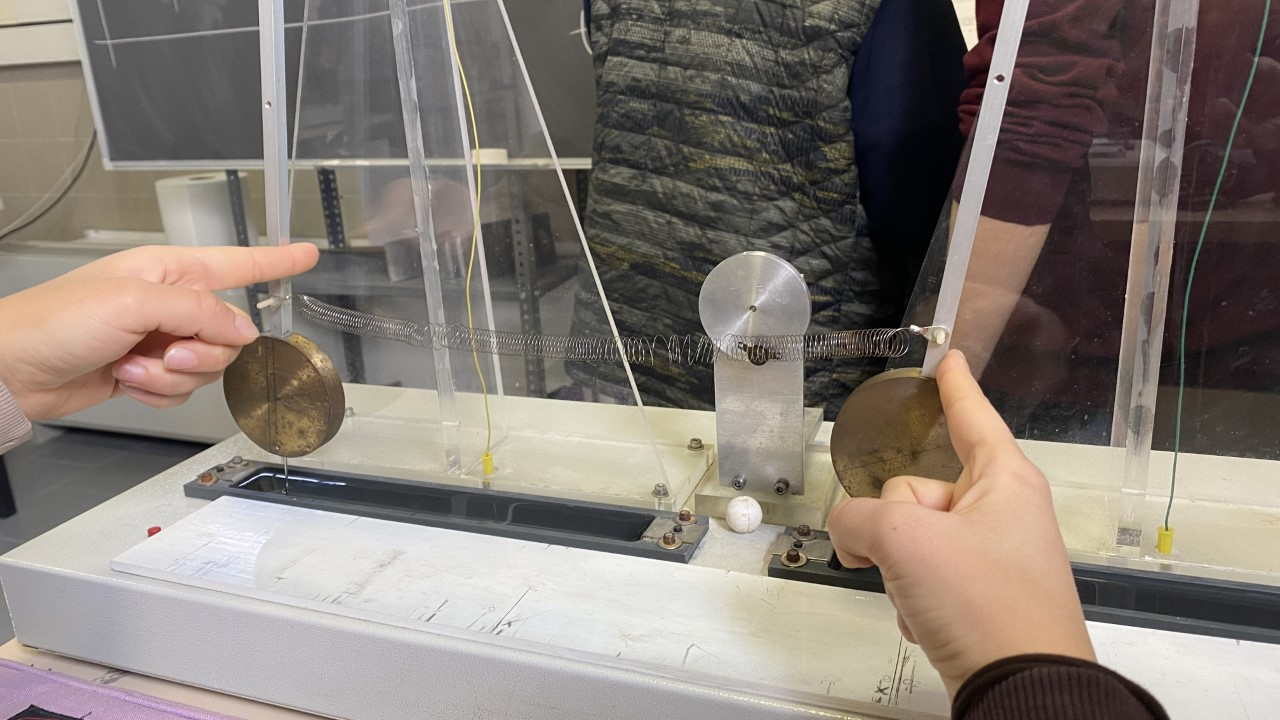
\includegraphics[width=10cm]{fase.jpg}
    \caption{Oscillazione in fase}
    \label{fig:fase}
\end{figure}
\begin{figure} [H]
    \centering
    \includegraphics[width=10cm]{controfase.jpg}
    \caption{Oscillazione in controfase}
    \label{fig:controfase}
\end{figure}
 Come si vede nelle figure \ref{fig:fase} e \ref{fig:controfase}, abbiamo spostato i pendoli della stessa ampiezza, nello stesso verso e in verso opposto rispettivamente per eccitare il sistema in modo che oscillasse in fase e in controfase. Per farlo, ci siamo servite di un pannello che era presente sotto l'apparato su cui segnare la distanza di allontanamento, in modo da essere più precise possibile per spostare i pendoli della stessa quantità.\\
 \\
Infine, abbiamo studiato il fenomeno dei battimenti. Per realizzare l'esperimento, abbiamo messo in oscillazione un pendolo lasciando fermo l'altro: lasciando oscillare il sistema con questa configurazione iniziale, si può notare come i due pendoli si scambino il moto, procedendo ad osservare che a tratti uno si ferma e l'altro è nella sua massima ampiezza di oscillazione e viceversa. \\
\\
Per quanto riguarda l'attribuzione delle incertezze, abbiamo
osservato il comportamento dei pendoli da fermi tramite il programma di acquisizione (che in uscita dà un file di quattro colonne di cui le prime due rappresentavano tempi e ampiezze per il pendolo A e le ultime due tempi e ampiezze per il pendolo B). Dal plot dei dati
sono ben distingubili diverse linee parallele all’asse x, da cui la deviazione standard delle
misure risulta essere dell’ordine di un'unità (per le ampiezze). Non abbiamo provato a fare stime più precise dato
che non disponevamo degli strumenti necessari per assicurarci che il pendolo fosse realmente fermo
entro la risoluzione strumentale.

\begin{figure} [H]
    \centering
    \includegraphics[width=15cm]{error.pdf}
    \caption{Plot delle misure acquisite per un pendolo fermo}
    \label{fig:my_label}
\end{figure}

Abbiamo invece assunto l'errore sui tempi pari alla risoluzione strumentale (cioè 0.001s). 
\vspace{1em}

\subsection{Analisi dei dati}
I dati raccolti sono stati analizzati tramite la funzione curve\_fit() di Python, realizzando così il grafico di best - fit ed il grafico dei residui. Un passo importante nell'analisi dei dati di ogni pendolo è stato assegnare valori di p guess ragionevoli alla funzione. Per farlo, abbiamo innanzitutto plottato i punti sperimentali su una griglia di matplotlib dalla quale potessimo valutare le coordinate dei vari punti. In tutti i casi abbiamo scartato una certa quantità di punti iniziali poichè i pendoli sono stati lasciati andare alcuni istanti dopo l'inizio di presa dati da parte del programma. Di seguito, per l'ampiezza A abbiamo preso la semi distanza tra il punto più basso e quello più alto; per il tempo di decadimento $\tau$ abbiamo valutato dopo quanti secondi l'ampiezza si fosse ridotta di circa $\frac{1}{3}$; per la pulsazione $\omega$ abbiamo assegnato il valore ottenuto da $\frac{2\pi}{T}$, dopo aver fatto una stima del periodo; per l'angolo iniziale di sfasamento $\phi$, considerando che la funzione di fit è cosinusoidale abbiamo valutato di quanto il primo punto fosse sfasato rispetto a un punto facilmente riconoscibile nell'andamento di una cosinusoide (e.g. quando cos $\theta$ = 0 o 1); infine, per la traslazione C abbiamo preso la distanza tra lo zero e il valore centrale dell'oscillazione. Sia per l'oscillazione senza smorzatore, sia per quella con smorzatore, che per i pendoli in fase e controfase la legge di fit utilizzata è:

\begin{equation}
    \theta(t) = Ae^{\frac{-t}{\tau}}cos(\omega t + \phi) + C
    \label{pendolo singolo}
\end{equation}

Dall'analisi risultano i seguenti grafici e parametri di best - fit:

\begin{figure} [H]
    \centering
    \includegraphics[width=15cm]{simple.pdf}
    \caption{Grafico di best fit per l'oscillazione del pendolo senza smorzatore}
    \label{fig:my_label}
\end{figure}

\begin{center}
\begin{tabular}{cc}
    \toprule
    Grandezze per il pendolo senza smorzatore & Misure \\
     \midrule
    A & $248.2 \pm 0.7$ u.a.\\
    $\tau$ & $51.0 \pm 0.3$ s\\
    $\omega$ & $4.4413 \pm 0.0001$ rad/s\\
    $\phi$ & $1.818 \pm 0.003$ rad\\
    C & $505.5 \pm 0.2$ u.a.\\
    $\chi^2$ & 37088 / 1029 dof\\
    T & $1.41266 \pm 5e-05$ s \\
    \bottomrule
\end{tabular}
\end{center}
\\
\vspace{1em}
Di seguito, abbiamo realizzato il fit dell'oscillazione del pendolo singolo con smorzatore, utilizzando gli stessi accorgimenti sopra elencati per assegnare ragionevoli valori di p guess:

\begin{figure} [H]
    \centering
    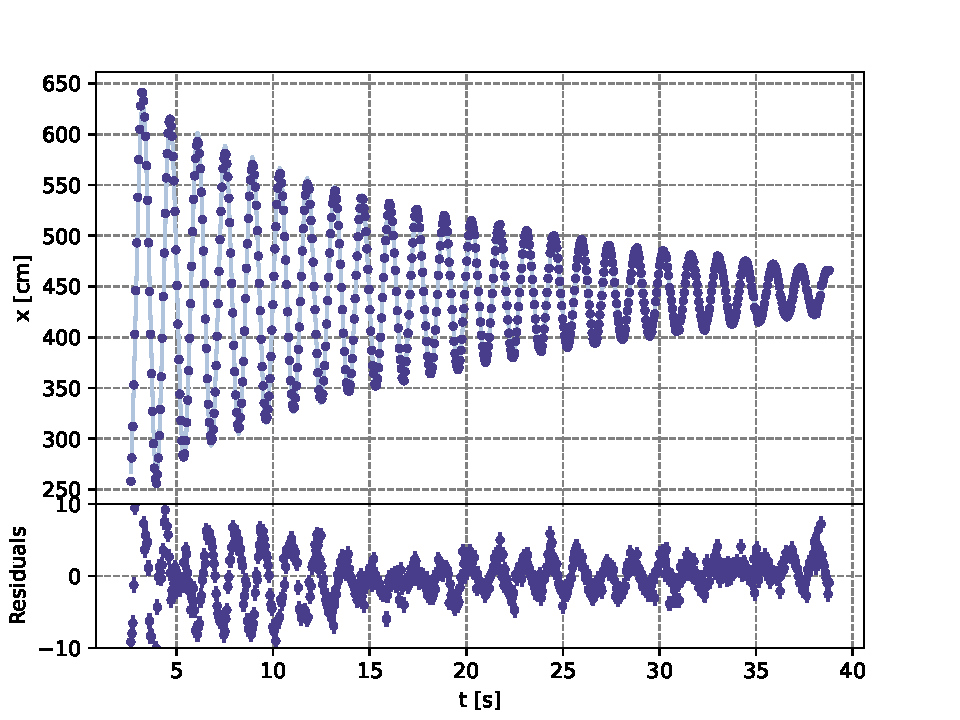
\includegraphics[width=15cm]{muted.pdf}
    \caption{Grafico di best fit per l'oscillazione del pendolo con smorzatore}
    \label{fig:my_label}
\end{figure}

\begin{center}
\begin{tabular}{cc}
    \toprule
    Grandezze per il pendolo senza smorzatore & Misure \\
     \midrule
    A & $210.8 \pm 0.6$ u.a.\\
    $\tau$ & $18.25 \pm 0.06$ s\\
    $\omega$ & $4.4305 \pm 0.0001$ rad/s\\
    $\phi$ & $-1.894 \pm 0.003$ rad\\
    C & $443.8 \pm 0.1$ u.a.\\
    $\chi^2$ & 2224 / 650 dof\\
    T & $1.41605 \pm 6e-05$ \\
    \bottomrule
\end{tabular}
\end{center}
\\
\vspace{1em}
Abbiamo poi condotto l'analisi dei modi normali (fase e controfase) tramite la stessa legge \eqref{pendolo singolo}, ottenendo i seguenti grafici e parametri di best fit:

\begin{figure} [H]
    \centering
    \includegraphics[width=12cm]{faseA.pdf}
    \caption{Grafico di best fit per l'oscillazione in fase del pendolo A}
    \label{fig:faseA}
\end{figure}

\begin{center}
\begin{tabular}{cc}
    \toprule
    Grandezze per il pendolo in fase A & Misure \\
     \midrule
    A & $266.6 \pm 1.3$ u.a.\\
    $\tau$ & $41.3 \pm 0.3$ s\\
    $\omega$ & $4.4340 \pm 0.0002$ rad/s\\
    $\phi$ & $0.800 \pm 0.005$ rad\\
    C & $405.8 \pm 0.3$ u.a.\\
    $\chi^2$ & 223289 / 1536 dof\\
    \bottomrule
\end{tabular}
\end{center}

\begin{figure} [H]
    \centering
    \includegraphics[width=12cm]{faseB.pdf}
    \caption{Grafico di best fit per l'oscillazione in fase del pendolo B}
    \label{fig:faseB}
\end{figure}

\begin{center}
\begin{tabular}{cc}
    \toprule
    Grandezze per il pendolo in fase B & Misure \\
     \midrule
    A & $232.5 \pm 1.4$ u.a.\\
    $\tau$ & $49.5 \pm 0.5$ s\\
    $\omega$ & $4.4431 \pm 0.0002$ rad/s\\
    $\phi$ & $0.687 \pm 0.006$ rad\\
    C & $507.2 \pm 0.3$ u.a.\\
    $\chi^2$ & 2068104 / 1536 dof\\
    \bottomrule
\end{tabular}
\end{center}
\\
\\
\begin{figure} [H]
    \centering
    \includegraphics{controA.png}
    \caption{Grafico di best fit per l'oscillazione in controfase del pendolo A}
    \label{fig:controA}
\end{figure}

\begin{center}
\begin{tabular}{cc}
    \toprule
    Grandezze per il pendolo in fase B & Misure \\
     \midrule
    A & $193.2 \pm 0.8$ u.a.\\
    $\tau$ & $38.6 \pm 0.2$ s\\
    $\omega$ & $4.6148 \pm 0.0002$ rad/s\\
    $\phi$ & $0.978 \pm 0.004$ rad\\
    C & $410.9 \pm 0.2$ u.a.\\
    $\chi^2$ & 90839 / 1989 dof\\
    \bottomrule
\end{tabular}
\end{center}

\begin{figure} [H]
    \centering
    \includegraphics{controB.png}
    \caption{Grafico di best fit per l'oscillazione in controfase del pendolo B}
    \label{fig:controB}
\end{figure}

\begin{center}
\begin{tabular}{cc}
    \toprule
    Grandezze per il pendolo in fase B & Misure \\
     \midrule
    A & $202.3 \pm 0.7$ u.a.\\
    $\tau$ & $37.4 \pm 0.2$ s\\
    $\omega$ & $4.6146 \pm 0.0001$ rad/s\\
    $\phi$ & $-2.152 \pm 0.004$ rad\\
    C & $551.4 \pm 0.2$ u.a.\\
    $\chi^2$ & 76314 / 1989 dof\\
    \bottomrule
\end{tabular}
\end{center}
\\
\vspace{1em}
Infine, abbiamo analizzato il fenomeno dei battimenti tramite la legge:

\begin{equation}
    \theta(t) = 2Ae^{-t/\tau}cos(\omega_1 t + \phi_1)cos(\omega_2 t + \phi_2) + C 
\end{equation}

ottenendo i seguenti grafici e parametri di best fit:

\begin{figure} [H]
    \centering
    \includegraphics[width=12cm]{beatsA.png}
    \caption{Grafico di best fit per i battimenti del pendolo A}
    \label{fig:my_label}
\end{figure}

\begin{center}
\begin{tabular}{cc}
    \toprule
    Grandezze per i battimenti del pendolo A & Misure \\
     \midrule
    A & $125.8 \pm 0.5$ u.a.\\
    $\tau$ & $42.1 \pm 0.2$ s\\
    $\omega_b$ & $0.0836 \pm 0.0002$ rad/s\\
    $\phi_b$ & $0.060 \pm 0.005$ rad\\
    $\omega_p$ & $4.5304 \pm 0.0001$ rad/s\\
    $\phi_p$ & $1.288 \pm 0.003$ rad\\
    C & $410.7 \pm 0.1$ u.a.\\
    $\chi^2$ & 39785 / 1443 dof\\
    \bottomrule
\end{tabular}
\end{center}

\begin{figure}[H]
    \centering
    \includegraphics[width=11cm]{beatsB.png}
    \caption{Grafico di best fit per i battimenti del pendolo B}
    \label{fig:my_label}
\end{figure}

\begin{center}
\begin{tabular}{cc}
    \toprule
    Grandezze per i battimenti del pendolo B & Misure \\
     \midrule
    A & $122.6 \pm 0.4$ u.a.\\
    $\tau$ & $42.6 \pm 0.2$ s\\
    $\omega_b$ & $0.1 \pm 8.7$ rad/s\\
    $\phi_b$ & $1.554 \pm 0.002$ rad\\
    $\omega_p$ & $4.5291 \pm 0.0001$ rad/s\\
    $\phi_p$ & $2.912 \pm 0.003$ rad\\
    C & $550.0 \pm 0.1$ u.a.\\
    $\chi^2$ & 19941 / 1443 dof\\
    \bottomrule
\end{tabular}
\end{center}

\vspace{2em}

\section{Conclusioni}
Per quanto riguarda l'oscillazione dei pendoli singoli, sono da fare alcune considerazioni:

\begin{itemize}
    \item è da notare innanzitutto come il valore ottenuto per $\omega$ del pendolo senza galleggiante non sia compatibile con quello che si ottiene a livello teorico dalla formula \eqref{omega}. Questo potrebbe essere spiegato dalle approssimazioni fatte sul momento d'inerzia del pendolo: avendo trascurato la massa dell'asta, abbiamo considerato il centro di massa del pendolo coincidente con il centro del cilindro; abbiamo inoltre anche approssimato il valore dell'accelerazione di gravità, nonchè supposto che il pendolo sia uniforme (quando in realtà sono presenti dei piccoli fori lungo l'asta) e le oscillazioni piccole;
    \item quanto ai periodi dei pendoli con e senza smorzatore, possiamo dire che dall'uno all'altro non cambi significativamente (infatti, differiscono per circa 4 millesimi di secondo);
    \item in ultima analisi, dai residui e dal valore del $\chi^2$ di entrambi i pendoli si può ipotizzare che il modello matematico utilizzato per descrivere il fenomeno non sia del tutto corretto. Infatti, per esempio, negli ultimi secondi dell'oscillazione smorzata si vede che la linea di fit prevede uno smorzamento minore di quello effettivo (e questo giustifica anche la poca concordanza modello - dati visibile sul grafico dei residui). Inoltre, è possibile ipotizzare che ci siano degli errori sistematici (che abbiamo omesso) dovuti all'apparato strumentale utilizzato (oltre all'errore strumentale stesso che abbiamo considerato), in particolare al modo in cui l'ago nell'acqua invia segnali al programma di acquisizione: in prossimità degli zeri della funzione l'ago è quasi totalmente immerso, mentre ai massimi e ai minimi può risultare anche quasi totalmente scoperto. Ciò implica, dunque, che lo strumento di acquisizione dati sovrastima e sottostima sistematicamente il valore centrale man mano che ci si allontana dalla posizione di equilibrio.
\end{itemize}
\\
Per ciò che concerne le oscillazioni in fase e controfase:
\begin{itemize}
    \item si nota subito dai valori ottenuti per le pulsazioni $\omega_{f(a)}, \omega_{f(b)}$ che non valga la condizione aspettata a livello teorico per la quale $\omega_f \sim \omega_0$; infatti, $\omega_{f(a)}$ e $\omega_{f(b)}$ non sono compatibili fra loro e non lo sono con $\omega_0$. Una possibile spiegazione è data dal fatto che abbiamo trascurato degli errori sistematici che fanno sì che l'incertezza sulla pulsazione sia almeno un ordine di grandezza più grande (come indicato nelle osservazioni esposte sopra), in aggiunta alla possibilità di non essere state estremamente precise nello spostare i pendoli della stessa quantità; tuttavia, in accordo con la teoria, dai dati analizzati risulta che $\omega_c > \omega_f$ e inoltre $\omega_{c(a)} \sim \omega_{c(b)}$;
    \item quanto all'andamento dei residui e al valore del $\chi^2$, è ragionevole supporre che valgano le stesse osservazioni precedentemente esposte;
    \item infine, possiamo dire di non essere riuscite a isolare completamente i
    due modi normali di oscillazione, come si evince dai grafici \ref{fig:faseA}, \ref{fig:faseB}, \ref{fig:controA}, \ref{fig:controB}: in alcuni intervalli di tempo si possono infatti osservare degli effetti di risonanza dovuti alla sovrapposizione del modo normale opposto a quello che si è cercato di isolare. Questo effetto è dovuto probabilmente al non essere state in grado di spostare i pendoli della stessa ampiezza (causa anche del mancato accordo tra $\omega_0, \omega_f$, come indicato sopra). Altra causa della risonanza può essere la molla di accoppiamento dei due pendoli, che risultava deformata agli estremi e nella zona centrale. 
\end{itemize}
\\
In ultima analisi, è possibile fare delle osservazioni sui battimenti:
\begin{itemize}
    \item come atteso dal modello teorico, l'oscillazione modulante di entrambi i pendoli è molto più piccola delle pulsazioni dei modi normali; per quanto riguarda invece l'oscillazione portante, è possibile vedere come, differentemente da come ci si aspettava dal modello teorico, esse non siano compatibili con le pulsazioni dei modi normali; ancora una volta, questo effetto può esser dovuto dalle cause sopra elencate;
    \item allo stesso modo di come illustrato sopra, il grafico dei residui e il valore del $\chi^2$ possono mostrare una mancata considerazione di errori sistematici rilevanti.
\end{itemize}
\\
\\
In conclusione, possiamo dirci soddisfatte per alcuni aspetti dell'esperienza, che però senz'altro risente di alcuni errori sistematici dei quali non si è potuto tenere conto. Un modo per minimizzare l'impatto di tali effetti avrebbe potuto essere considerare l'oscillazione solo per intervalli ristretti ed in particolare per i dati finali di ogni acquisizione (laddove le oscillazioni si fanno più piccole e i dati sembrano trovarsi maggiormente in accordo con il modello teorico), cosa che però non vale per l'oscillazione smorzata con galleggiante (poichè evidentemente non abbiamo utilizzato un modello propriamente corretto).
\end{document}
